\section{Construcción y Manufactura}

La fabricación del cohete PDA STARS se basó en una estrategia híbrida que combina la ligereza del tubo Kraft enrollado en espiral con la precisión dimensional y rigidez mecánica de la manufactura aditiva FDM en filamentos de ingeniería.

\subsection{Diseño y Planificación de la Construcción}
Se generó el despiece computacional a partir de los modelos validados en OpenRocket y Fusion 360, estableciendo tolerancias de ajuste deslizante suave ($0,15\text{ -- }0,20\text{ mm}$) en la unión de la ojiva y la bahía de carga útil para evitar tanto el desacople prematuro por vibración como el bloqueo durante la sobrepresión de eyección.

\begin{figure}[H]
\centering
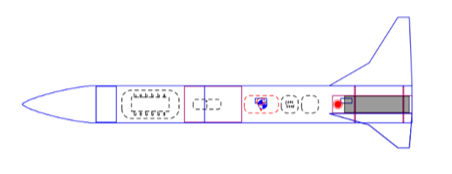
\includegraphics[width=0.85\linewidth]{diseno_openrocket.png}
\caption{Modelo geométrico y esquema de distribución interna en OpenRocket.}
\label{fig:openrocket_layout}
\end{figure}

\subsection{Modelado 3D de Componentes Estructurales}
Las aletas, anillos de centrado y acoples fueron diseñados con ranuras pasantes a través del fuselaje (\textit{through-the-wall}) para crear una unión monolítica entre el fuselaje Kraft y el tubo portamotor concéntrico de 29 mm.

\begin{figure}[H]
\centering
\begin{subfigure}[b]{0.45\linewidth}
    \centering
    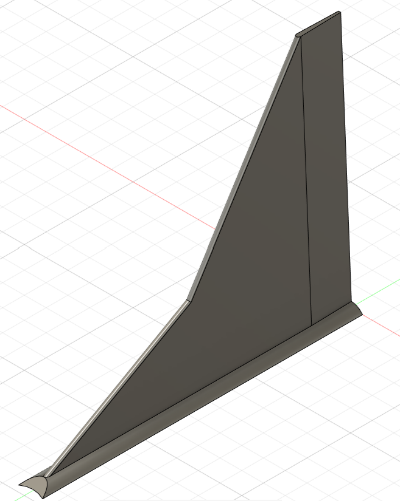
\includegraphics[height=3.5cm,keepaspectratio]{cad_aleta.png}
    \caption{Aleta en PETG-CF.}
\end{subfigure}
\hfill
\begin{subfigure}[b]{0.45\linewidth}
    \centering
    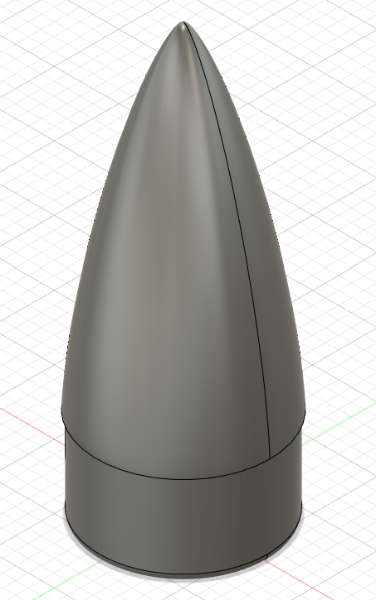
\includegraphics[height=3.5cm,keepaspectratio]{cad_ojiva.png}
    \caption{Ojiva Haack.}
\end{subfigure}
\vspace{0.3cm}
\begin{subfigure}[b]{0.45\linewidth}
    \centering
    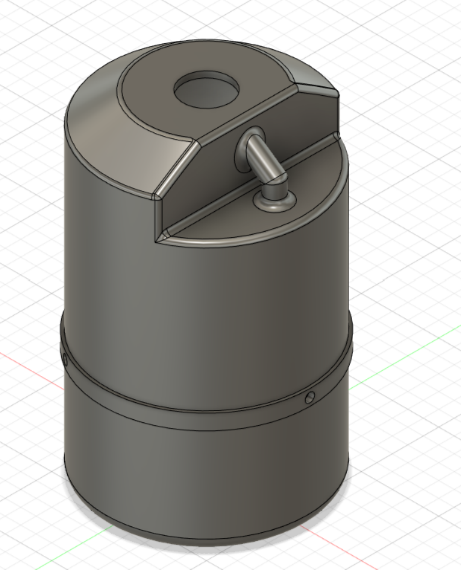
\includegraphics[height=3.5cm,keepaspectratio]{cad_acople.png}
    \caption{Acople con ojal.}
\end{subfigure}
\hfill
\begin{subfigure}[b]{0.45\linewidth}
    \centering
    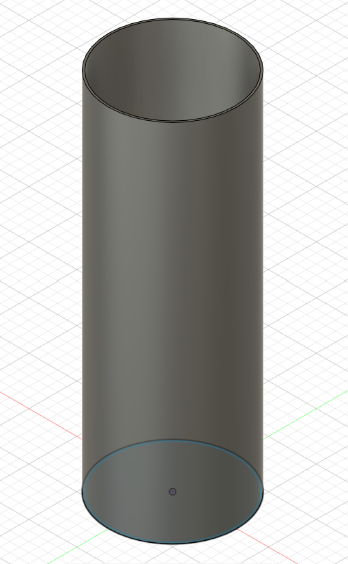
\includegraphics[height=3.5cm,keepaspectratio]{cad_centrador.png}
    \caption{Anillo de centrado.}
\end{subfigure}
\caption{Componentes modelados en CAD para manufactura aditiva FDM.}
\label{fig:cad_piezas}
\end{figure}

\subsection{Selección de Materiales y Criterio Técnico}
\begin{figure}[H]
\centering
\begin{subfigure}[b]{0.48\linewidth}
    \centering
    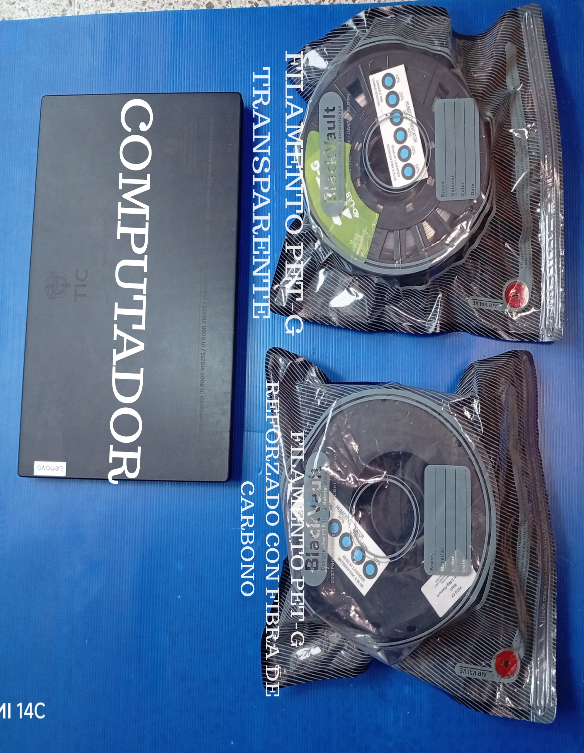
\includegraphics[height=4.5cm,keepaspectratio]{filamentos.png}
    \caption{Filamentos técnicos PETG y PETG-CF.}
\end{subfigure}
\hfill
\begin{subfigure}[b]{0.48\linewidth}
    \centering
    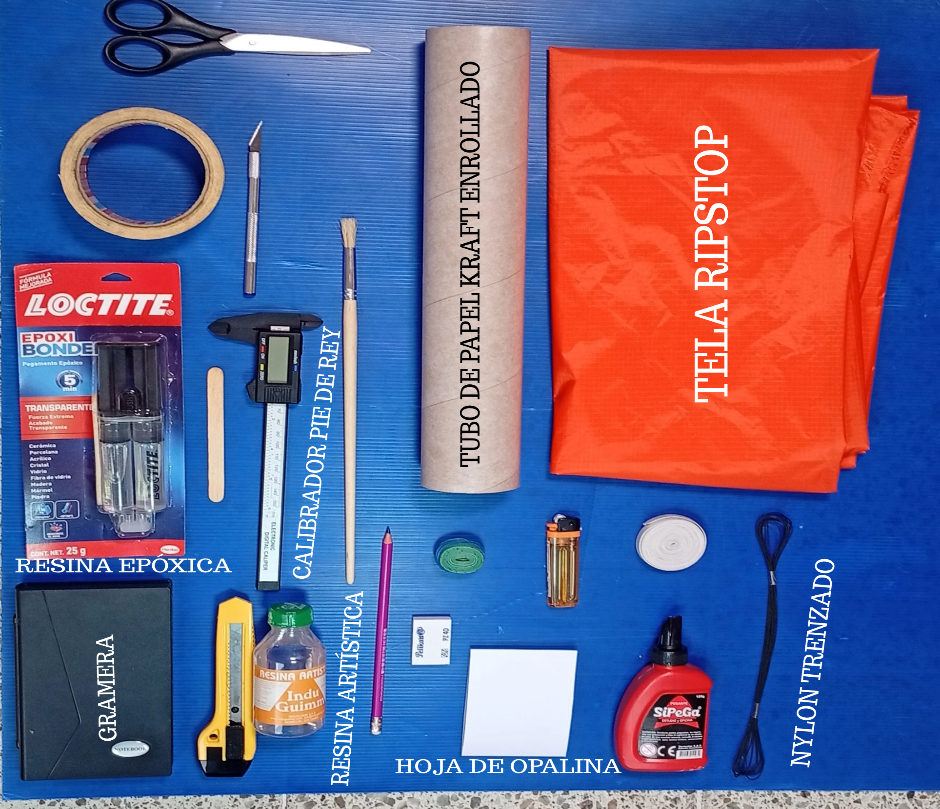
\includegraphics[height=4.5cm,keepaspectratio]{materiales.png}
    \caption{Materiales compuestos, epoxi y fuselaje.}
\end{subfigure}
\caption{Materiales seleccionados para la construcción de PDA STARS.}
\label{fig:materiales_utilizados}
\end{figure}

\begin{itemize}[leftmargin=1.5em]
    \item \textbf{PETG Estándar (Ojiva):} Empleado en la ojiva y carcasa de la carga útil para garantizar \textbf{permeabilidad electromagnética total} y evitar el efecto jaula de Faraday sobre las lecturas y antenas de telemetría.
    \item \textbf{PETG Reforzado con Fibra de Carbono (PETG-CF):} Utilizado exclusivamente en aletas y anillos de centrado por su módulo de elasticidad superior ($> 4,5\text{ GPa}$) y resistencia térmica ante gases de escape del motor F15.
    \item \textbf{Tubo Kraft Fenólico BT-80:} Ofrece alta resistencia específica a compresión y flexión con masa volumétrica reducida frente a tubos plásticos comerciales.
\end{itemize}

\subsection{Proceso de Fabricación y Ensamble}
\begin{figure}[H]
\centering
\begin{subfigure}[b]{0.48\linewidth}
    \centering
    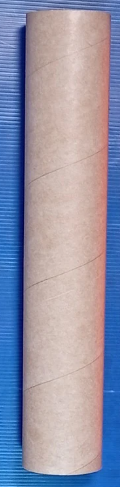
\includegraphics[height=4.2cm,keepaspectratio]{tubo_recibido.png}
    \caption{Corte y calibración de tubos Kraft BT-80.}
\end{subfigure}
\hfill
\begin{subfigure}[b]{0.48\linewidth}
    \centering
    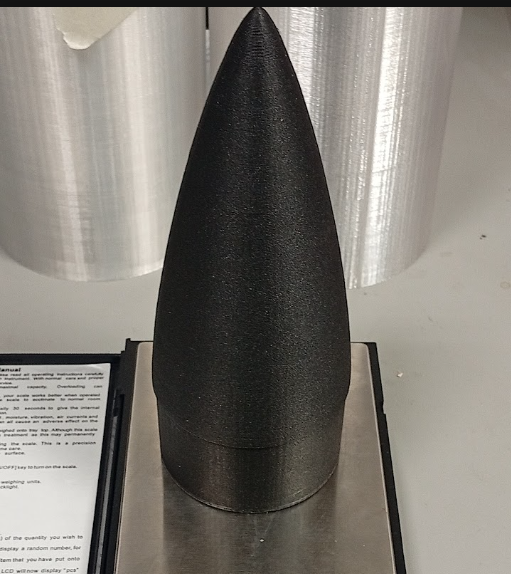
\includegraphics[height=4.2cm,keepaspectratio]{ojiva_impresa.png}
    \caption{Ojiva impresa en PETG con acabado pulido.}
\end{subfigure}
\caption{Mecanizado de fuselaje y manufactura aditiva de la ojiva.}
\label{fig:fabricacion_piezas}
\end{figure}

\begin{figure}[H]
\centering
\begin{subfigure}[b]{0.48\linewidth}
    \centering
    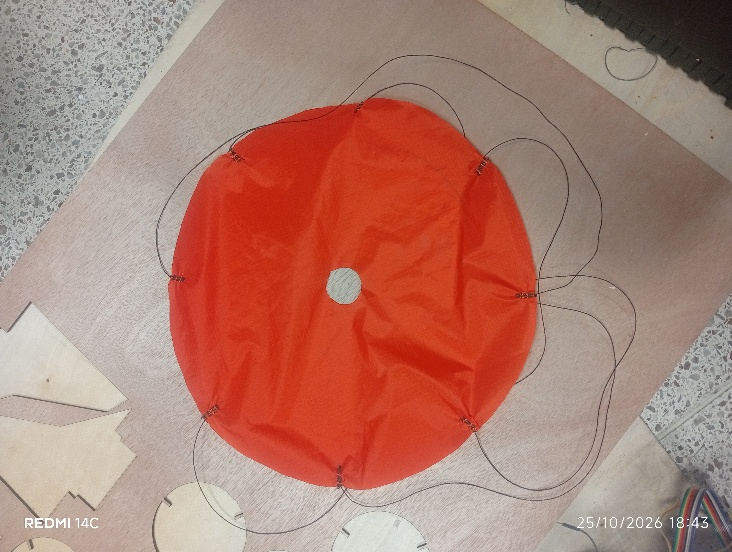
\includegraphics[height=4.2cm,keepaspectratio]{paracaidas_fisico.jpg}
    \caption{Paracaídas de 40 cm en tela ripstop con 8 líneas.}
\end{subfigure}
\hfill
\begin{subfigure}[b]{0.48\linewidth}
    \centering
    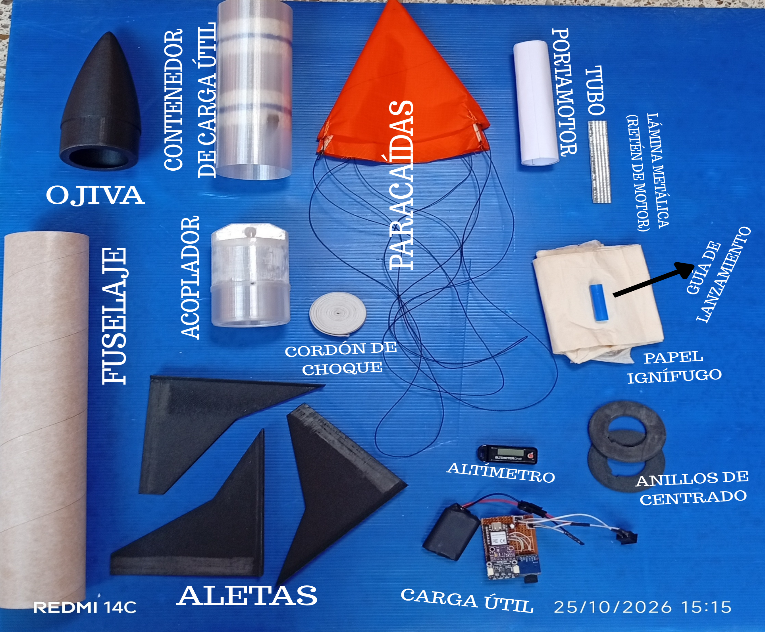
\includegraphics[height=4.2cm,keepaspectratio]{partes_sin_ensamblar.png}
    \caption{Inspección previa de componentes físicos listos.}
\end{subfigure}
\caption{Sistema de recuperación y verificación previa al ensamble estructural.}
\label{fig:componentes_previos}
\end{figure}

\begin{figure}[H]
\centering
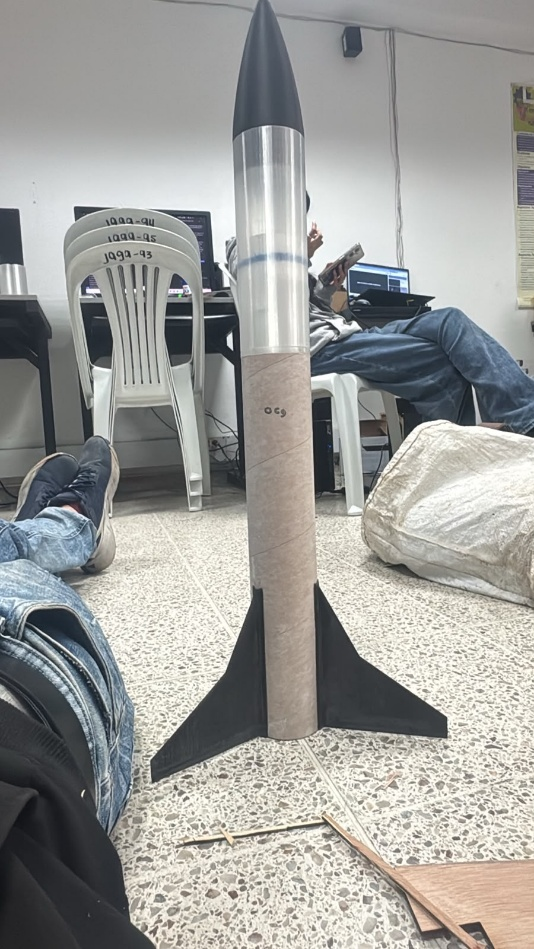
\includegraphics[height=7.0cm,keepaspectratio]{cohete_terminado.jpg}
\caption{Cohete PDA STARS completamente ensamblado en taller.}
\label{fig:cohete_terminado}
\end{figure}

\subsection{Balance de Masas Final}
\begin{table}[H]
\centering
\small
\begin{tabularx}{\linewidth}{Xccc}
\toprule
\rowcolor{navyiejaga!15}
\textbf{Subconjunto / Componente} & \textbf{Masa Teórica (ORK)} & \textbf{Masa Real Taller} & \textbf{Desviación} \\
\midrule
Ojiva Haack PETG & 39,7 g & 41,2 g & $+3,8\%$ \\
\rowcolor{grisclaro}
Bahía y contenedor de carga útil & 60,0 g & 60,0 g & $0,0\%$ (Cumple $\le 60\text{ g}$) \\
Instrumentación electrónica y batería & 9,9 g & 10,5 g & $+6,0\%$ \\
\rowcolor{grisclaro}
Fuselaje principal Kraft BT-80 & 30,0 g & 31,4 g & $+4,6\%$ \\
Conjunto de 3 aletas en PETG-CF & 64,0 g & 63,8 g & $-0,3\%$ \\
\rowcolor{grisclaro}
Portamotor 29 mm y centradores & 14,0 g & 14,6 g & $+4,2\%$ \\
Paracaídas 40 cm, manta Nomex y Kevlar & 11,0 g & 11,5 g & $+4,5\%$ \\
\rowcolor{grisclaro}
Adhesivo epóxico y acabados & 53,5 g & 54,0 g & $+0,9\%$ \\
\midrule
\textbf{Masa total en seco (Dry Mass)} & \textbf{282,1 g} & \textbf{287,0 g} & $+1,7\%$ \\
\rowcolor{grisclaro}
Motor Estes F15-4 cargado & 91,0 g & 91,0 g & $0,0\%$ \\
Instrumentación complementaria en rampa & 150,0 g & 150,0 g & $0,0\%$ \\
\midrule
\rowcolor{navyiejaga!10}
\textbf{Masa total en rampa (Liftoff Mass)} & \textbf{523,1 g} & \textbf{528,0 g} & $\mathbf{+0,9\%}$ (Límite $< 650\text{ g}$) \\
\bottomrule
\end{tabularx}
\caption{Balance de masas estimado vs medido en báscula digital de precisión.}
\label{tab:balance_masas}
\end{table}
